\documentclass[]{article}
\usepackage[UTF8]{ctex}
\usepackage[a4paper,left=10mm,right=10mm,top=10mm,bottom=10mm]{geometry}
\usepackage{amsmath,amsfonts,amssymb,amsthm}
\usepackage{float}
\usepackage{graphicx}

%opening
\title{计算机科学中的数学基础W2-2}
\author{陈昱衡 521021910939}

\begin{document}

\maketitle



\section*{Warmup6}
\begin{figure}[hbt]
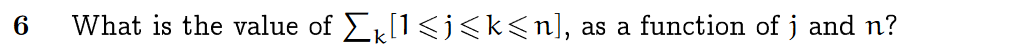
\includegraphics[scale=1]{Q1}
\end{figure}
根据艾弗森约定,该合式是对所有满足 $1 \le j \le k \le n$ 的整数k的个数。\par 
因此,由如下讨论:
\[ sum = \left\{ \begin{array}{rl} 0 & \text{if } j < 1 或 j > n,\\ n - j + 1 & \text{otherwise}  \end{array} \right. \]




\section*{Basics11}
\begin{figure}[hbt]
	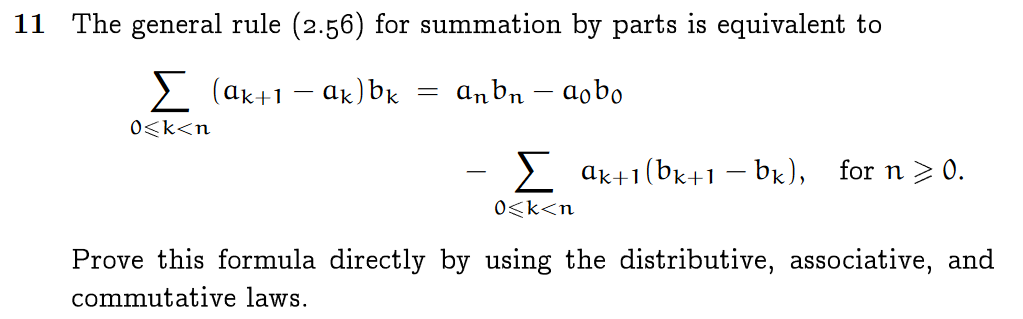
\includegraphics[scale=1]{Q3}
\end{figure}
为了证明这个等式,等价于证明:
\begin{equation}
	\sum_{0 \le k < n} (a_{k+1} - a_{k})b_{k} + \sum_{0 \le k < n}a_{k+1}(b_{k+1} - b_{k}) = a_{n}b_{n} - a_{0}b_{0}
\end{equation}

对等式左侧使用分配律:
\begin{equation}
	\sum_{0 \le k < n} (a_{k+1} - a_{k})b_{k} + \sum_{0 \le k < n}a_{k+1}b_{k+1} - \sum_{0 \le k < n}a_{k+1}b_{k} 
\end{equation}

继续使用结合律:
\begin{equation}
	\sum_{0 \le k < n} (a_{k+1} - a_{k} -a_{k+1})b_{k} + \sum_{0 \le k < n}a_{k+1}b_{k+1}
\end{equation}
即:
\begin{equation}
	\sum_{0 \le k < n}- a_{k}b_{k} + \sum_{0 \le k < n}a_{k+1}b_{k+1}
\end{equation}
使用结合律:
\begin{equation}
	\sum_{1 \le k \le n-1} (a_{k}b_{k} - a_{k}b_{k})  + a_{n}b_{n} - a_{0}b_{0}
\end{equation}
即:
\begin{equation}
	 a_{n}b_{n} - a_{0}b_{0}
\end{equation}
得到等式右侧,证毕。

\section*{Basics12}
\begin{figure}[H]
	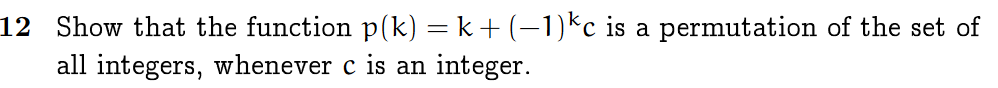
\includegraphics[scale=1]{Q2}
\end{figure}
我们可以取一对整数m,n,满足$p(m) = p(n) - 1$。不是一般性,不妨约定m为奇数,n为偶数,得到m和n的关系式:m = n + 2c - 1,该等式刻画的m,n关系满足约定。\par 
由此,取数列{$\cdots$ ,m-2 , m, m+2,$\cdots$},{$\cdots$,n-2,n,n+2,$\cdots$ },因为m,n在函数p作用下映射为两个连续的数,因此,由以上两个数列产生的数字也相邻,由此得到了关于整数集的一一映射关系。\par 
即可以得出结论:函数p是整数集的一个全排列。

\section*{Basics13}
\begin{figure}[H]
	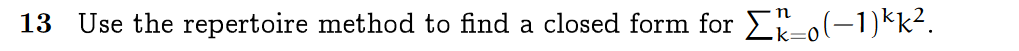
\includegraphics[scale=1]{Q4}
\end{figure}
% 我们不妨令$S_{n} = \sum_{k=0}^{n} k^2  $。
% 根据题意,我们可以得到等式:$S_{n} = S_{n-1} + (-1)^n n^2$。
% 由成套方法,我们不妨假设$S_{n} = A(n)\alpha + \beta$。\par 
由题意,我们可以设:
\begin{align}
	S_{n} &= S_{n-1} + (-1)^n(\beta+n\gamma=n^2\eta)  \\
	S_{0} &= \alpha
\end{align}
由成套方法,我们可以令:
\begin{align}
	S_{n} &= A(n)\alpha + B(n)\beta + C(n)\gamma + D(n)\delta \\
	S_{0} &= \alpha\\
\end{align}
由成套方法的分析过程,我们首先令:
\begin{equation}
	S_{n} = 1
\end{equation}
得到,
\begin{equation}
	A(n) = 1
\end{equation}
再令:
\begin{equation}
	S_{n} = (-1)^n
\end{equation}
得到,
\begin{equation}
	A(n)+2B(n) = (-1)^n
\end{equation}
再令:
\begin{equation}
	S_{n} = (-1)^n n^2
\end{equation}
得到,
\begin{equation}
	B(n)-2C(n)+2D(n) = (-1)^n n^2
\end{equation}
由以上三个方程,我们可以得到:
\begin{equation}
	2D(n) = (-1)^n (n^2+n)
\end{equation}
由此,我们可以得到:
\begin{equation}
	D(n) = \frac{(-1)^n (n^2+n)}{2}
\end{equation}
\end{document}
